\section{Introduction}
\\
\\
\\
\begin{center}
    \textit{<<In the twenty-first century the \\
    robot will take the place which \\
    slave labor occupied in ancient \\ 
    civilization. There is no reason at \\ 
    all why most of this should not \\
    come to pass in less than a century, \\
    freeing mankind to pursue its \\
    higher aspirations.>>} \\ 
            \text{Nikola Tesla (1856 - 1943) }
\end{center}


\begin{center}
    \textit{<<Robots of the world! \\
    The power of
man has fallen!\\ A new world has
arisen:\\ the Rule of the Robots!
March!>>}\\
    \text{Rossum's Universal Robot (1920)}
\end{center}

Man has always spent his life working. Dangerous and degrading work has been the cause of death for many people for centuries. 
In this sense, there has always been a tendency to try to relieve man of the heaviest jobs by looking for machines or automatic systems to replace him.
In a sense, with the advent of the industrial revolution, we witnessed the first real process of robotizing in history.
On the other hand, with the evolution of discoveries in the medical field, the desire and curiosity arose in man to try to clone himself, artificially constructing his own like.
It is here that these two needs and tendencies come together in what we now call humanoid robots.
Indeed, humanoid robots are designed and built to replace humans in the most physical and repetitive tasks, in order to ensure greater well-being.

\newpage

\section{History of Robotics}
In recent years, the general public has become increasingly interested in robots and robotics research. New developments, e.g. robotic competitions, which "push beyond the boundaries of current technological
systems" (such as Defense Advanced Research Projects Agency (DARPA) in the
United States), especially in the area of robotics, have promised and delivered
fully integrated systems, \citet{robocomp}.\\
But the idea of creating intelligent, useful machines for humans has existed since the beginning of mankind.
In fact, ever since civilisation, one of the most unattainable desires and ambitions for mankind has been to create artifacts of his own image.\\
From a historical perspective, the first example that can be interpreted as such dates back to 3500 B.C., with the legend of the giant Talus, the slave forged by Hephaestus.
Continuing in time and reaching the Babylonians in 1400 B.C., we can observe the creation of the first automatic machine, the clepsydra water clock.
Continuing through the centuries, creations became more and more technologically advanced and jumping back to the 1500s, we encounter Leonardo da Vinci and his many inventions.
\begin{figure}[H]
    \centering
    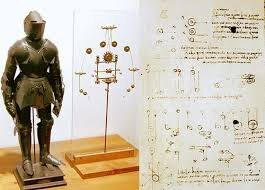
\includegraphics{Chapter 3/davinchiknight.jpeg}
    \caption{Leonardo da Vinci’s mechanical knight: sketches on the right, rebuilt
and showing its inner workings on the left.}
    \label{fig:my_label}
\end{figure}
The concept of the robot then gradually entered people's minds thanks to this long process, but it was only in the 20th century that it took on a real physical connotation.
\newline
The term 'robot' was introduced in 1920 by the play 'Rossum's Universal Robot', by Karel Čapek: it derives etymologically from the Slavic root word 'robota' meaning subordinate labor.
\begin{figure}[H]
    \centering
    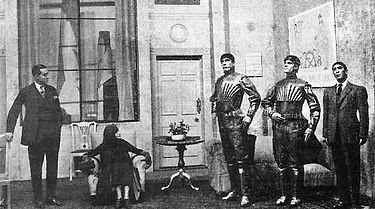
\includegraphics{Images/Chapter 3/rossumplay.jpg}
    \caption{A scene from Rossum's Universal Robot play, showing three robots}
    \label{fig:rossum}
\end{figure}
Later, during the middle of the century, the first research into the connection between human and machine intelligence was undertaken, marking the beginning of Artificial Intelligence (AI).
Between 1950 and 1980, Isaac Asimov wrote the so called "Three Laws of Robotics" in his book 'Runaround'. They are encoded in the "positronic brains" and are defined as follows, \citet{asimov}:
\begin{itemize}
\item A robot may not injure a human being or, through inaction, allow a human
being to come to harm.
\item A robot must obey the orders given to it by human beings, except where
such orders would conflict with the First Law.
\item A robot must protect its own existence as long as such protection does not
conflict with the First or Second Law.
\end{itemize}
Around those years, the first robots were created, they stemmed from the confluence of advances in two fields: numerically controlled machines for precision manufacturing and remote control to handle highly radioactive materials.
In fact, these two fields already featured modern applications of technologies such as mechanics, control, computational science and electronics.
The first robots were therefore master-slave arms, designed to reproduce the mechanics of the human arm but with rudimentary control and little perception.\\
During the second half of the century, the development of integrated circuits, digital computers and miniaturised components allowed terminal-controlled robots to be designed and developed.\\
In fact, in the 1980s, robotics was defined as the science that studies the connection between action and perception.In fact, action involves a locomotion apparatus that moves in the environment and a manipulation apparatus that performs actions, modifying its surroundings, thanks to special actuators and end-effectors.\\
Perception is then extracted from the sensors that provide information about the state of the robot (e.g. position and speed) and its surroundings (e.g. range and vision).
In the 1990s, research was further accelerated by the need to rely on robots to replace human presence in critical environments.\\
As we enter the new millennium, robots have undergone profound transformations both in their scope of use and in their shapes and sizes. 
\subsubsection{Humanoid Robots}
As reported in the article "Humanoid Robots:Historical Perspective, Overview and Scope", \citet{Siciliano2020}:\\
\\
"\textit{The long saga of humanoid robots in science fiction has influenced generations
of researchers, as well as the general public, and serves as evidence that people
are drawn to the idea of humanoid robots. Humans generally like to observe and
interact with one another. In their social behavior, people are highly attuned to
human characteristics, such as the sound of human voices and the appearance of
human faces and body motion. \\
Infants show preferences for these types of stimuli at
a young age, and adults appear to use specialized mental resources when interpreting these stimuli. By mimicking human characteristics, humanoid robots can engage
these same preferences and mental resources.\\
Throughout history, the human body and mind have inspired artists, engineers,
and scientists, using media as diverse as cave paintings, sculpture, mechanical toys,
photographs, and computer animation. \\
Humanoid robots serve as a powerful new
medium that enables the creation of artifacts that operate within the real world
and exhibit both human form and behavior. 
\\The field of humanoid robotics focuses
on the creation of robots that are directly inspired by human capabilities and/or
selectively imitate aspects of human form and behavior. Humanoids come in a
variety of shapes and sizes, from complete human-size legged robots to isolated
robotic heads with human-like sensing and expression.}"\\
Thus, humanoid robots were developed to be employed as multi purpose mechanical workers, and were designed to work alongside humans in daily tasks, being a support, living in the same environment and using the same tools.
It must also be considered that when the robot moves around in the work environment, there can be multiple risks for the worker; in this respect, a subfield of robotics, called cognitive robotics, has taken hold.
Indeed, robots can take advantage of the traditional communication methods used among humans to become more aware of their surroundings.
An even more ambitious aim is to interpret human gestures through vision (eye gaze, body language). On the other hand, this could put a human in a difficult relationship with the robot, modelled by the phenomenon called 'uncanny valley', a concept introduced in the 1970s by Masahiro Mori, a professor at the Tokyo Institute of Technology.
Masahiro in fact argues that:\\
"\textit{I have noticed that, in climbing toward the goal of making robots appear human, our affinity for them increases until we come to a valley, which I call the uncanny valley.}"
\begin{figure}[H]
    \centering
    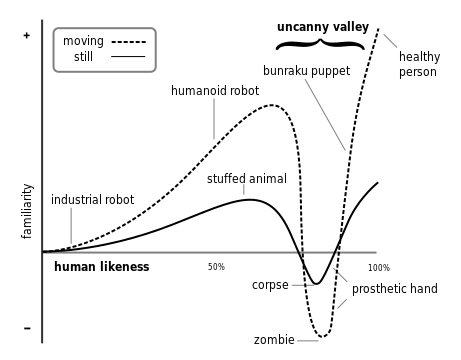
\includegraphics[scale=0.8]{Images/Chapter 3/Mori_Uncanny_Valley.png}
    \caption{Mori Uncanny Valley}
    \label{fig:mori_uncanny_valley}
\end{figure}
Mori better explains this concept with the example of the prosthetic hand:
\\
"\textit{One might say that the prosthetic hand has achieved a degree of resemblance to the human form, perhaps on a par with false teeth. However, when we realize the hand, which at first site looked real, is in fact artificial, we experience an eerie sensation. For example, we could be startled during a handshake by its limp boneless grip together with its texture and coldness. When this happens, we lose our sense of affinity, and the hand becomes uncanny.}"
\\
On the other hand, many scientists and researchers in the robotics community see humanoid robots as a possibility to better investigate human nature itself.
A part from the roles mentioned above, a humanoid robot could work as an avatar for telepresence, test ergonomics and serve for any other  roles that a human can do.
Even though in the past decades, humanoids have only been applied in research field, times seem to be mature to put these robots on field and let them cooperate with humans.
\section{Robee: Oversonic Robotics configuration}
In order to make physical sense of the results obtained within this project, it is important to define what technologies were used and what materials made up Robee's hardware.
\subsection{Hardware components and software architecture}
It is important to bear in mind that the Oversonic project has an architecture split between the
robot (also referred to as the edge) and the cloud, and these two components coexist in a
hybrid.
Describing the system from the cloud, the hardware component consists of a scalable node pool based on
the 2.35Ghz AMD EPYC 7452 processor that can achieve a boosted maximum frequency
of 3.35GHz with 32 GB RAM memory, running a Kubernetes instance on top of Linux
Ubuntu 18.04 (Bionic Beaver).
As far as the robot is concerned, all the computational power is provided by 2 Intel NUCs 8 including an Intel Core i5-8259U Processor (6M Cache, up to 3.80 GHz), 8 GB RAM and Integrated Graphics Intel Iris Plus 655.
The operating system which is mounted on is Linux Ubuntu 20.04 (Focal Fossa), and all the modules are running containers that on turn are managed by KubeEdge, a containers orchestration system built on Kubernetes.
\begin{figure}[H]
    \centering
    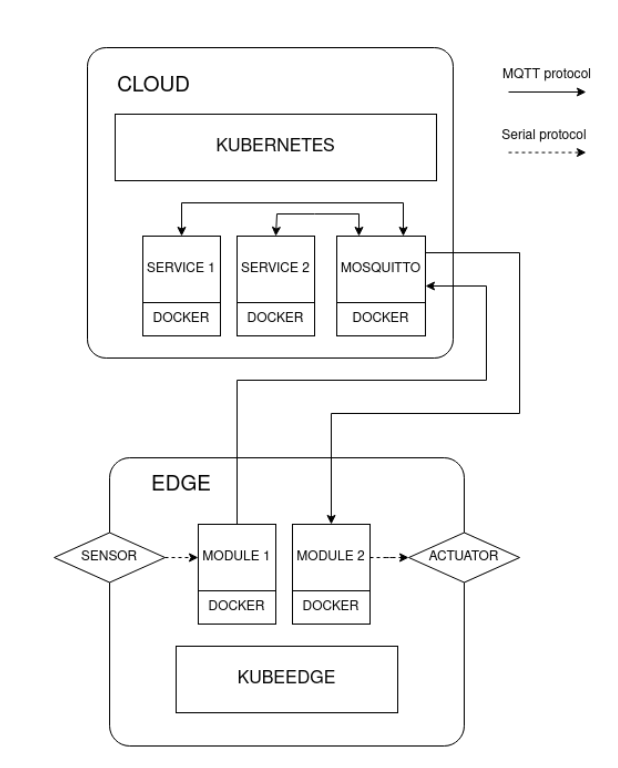
\includegraphics[scale=0.6]{Images/Chapter 3/oversonicarch.png}
    \caption{Oversonic Architecture}
    \label{fig:oversonicarch}
\end{figure}
\textbf{Internet of Things}\\
In the case of the Robee project, the architecture is therefore composed of various software modules that are containerised and must be able to communicate with each other.
The MQTT protocol is an optimal choice for this case.\\
From the official MQTT.org site: "\textit{MQTT is an OASIS standard messaging protocol for
the Internet of Things (IoT). It is designed as an extremely lightweight publish/subscribe
messaging transport that is ideal for connecting remote devices with a small code footprint and minimal network bandwidth. MQTT today is used in a wide variety of industries, such as automotive, manufacturing, telecommunications, oil and gas}", \citet{mqtt}.\\
MQTT therefore operates at the application layer of the OSI model, relying on TCP at the transport layer.
The MQTT protocol establishes two kinds of entities in the network: a message broker and a number of clients. The broker is nothing more than a server that receives all messages from all clients and then routes these messages to the relevant destination clients. A client is anything that can interact with the broker to exchange messages. The messages are routed to clients basing
on topics: every message is published over a specific topic, and only the clients subscribed
to it will receive the message.\\ A client, therefore, can be an IoT sensor or an application in a data centre that processes IoT data.
Each MQTT message has a command and a payload. The command defines the type of message:
\begin{itemize}
    \item CONNECT: initial message sent from client to broker, to instantiate a new connection
    \item DISCONNECT: final message sent from client to broker to end the connection
    \item PUBLISH: command to publish a message over a specified topic, it is sent from client to broker and then routed from broker to every client that appears to be subscribed to that topic
    \item SUBSCRIBE: message sent from client to broker in order to request a subscription to a specified topic
\end{itemize}
All MQTT libraries provide simple ways to handle such messages directly and can automatically populate certain required fields, such as 'message' and 'client Id'.
\begin{figure}[H]
    \centering
    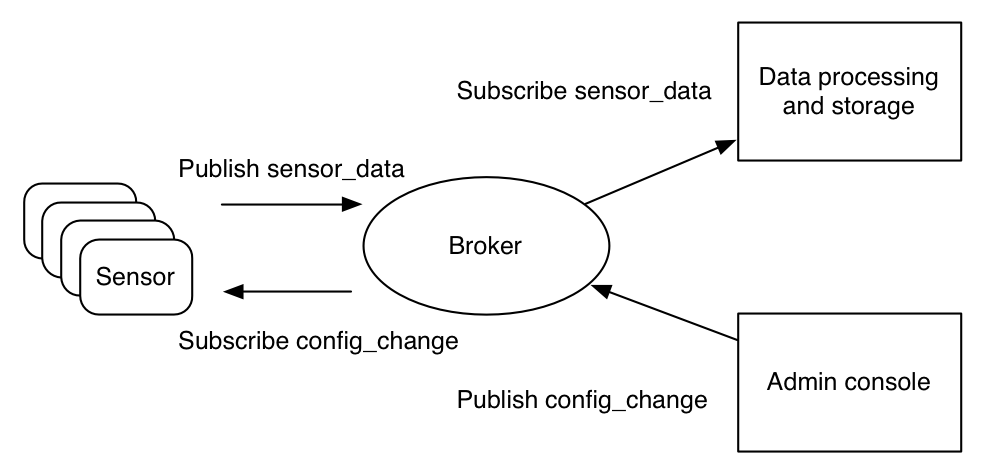
\includegraphics[scale = 0.8]{Images/Chapter 3/mqtt.png}
    \caption{The MQTT publish and subscribe model for IoT sensors}
    \label{fig:mqtt}
\end{figure}
\subsection{Kinematics Configurations}
    SOLO DIFFERENTIAL DRIVE DI ROBEE E AMBROGIONE O ANCHE SKID STEERING DI AMBROGINO?
    EQUAZIONI!!!

\subsection{Sensors}
INTRO AI SENSORI 
-> CAMERE UTILIZZATE D400 E T265
\newpage
POINTCLOUD?

\newpage
-> BEACON?
-> APRILTAG?
